\appendix
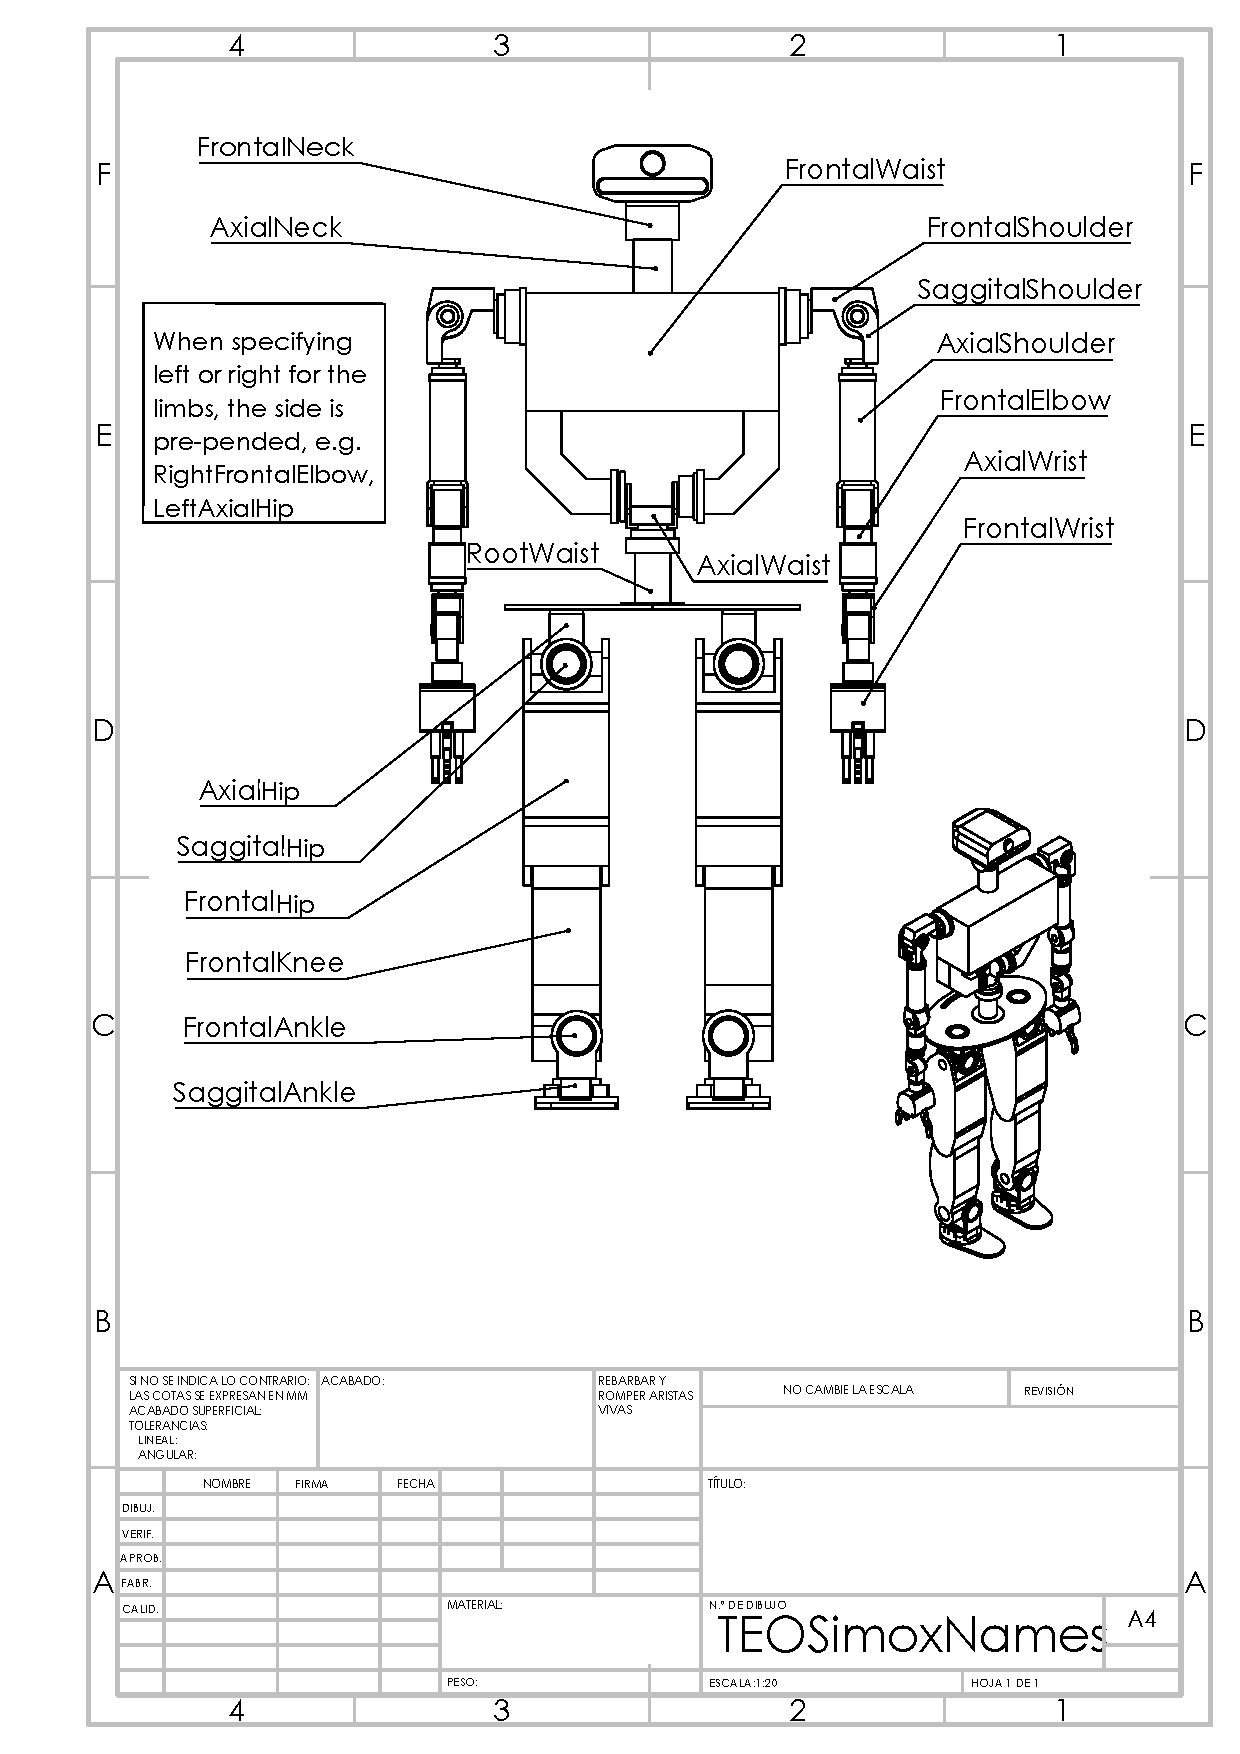
\includepdf[scale=0.8,pagecommand=\section{Estructura del robot TEO}\label{aped.A}]{apendices/teo-link-names}



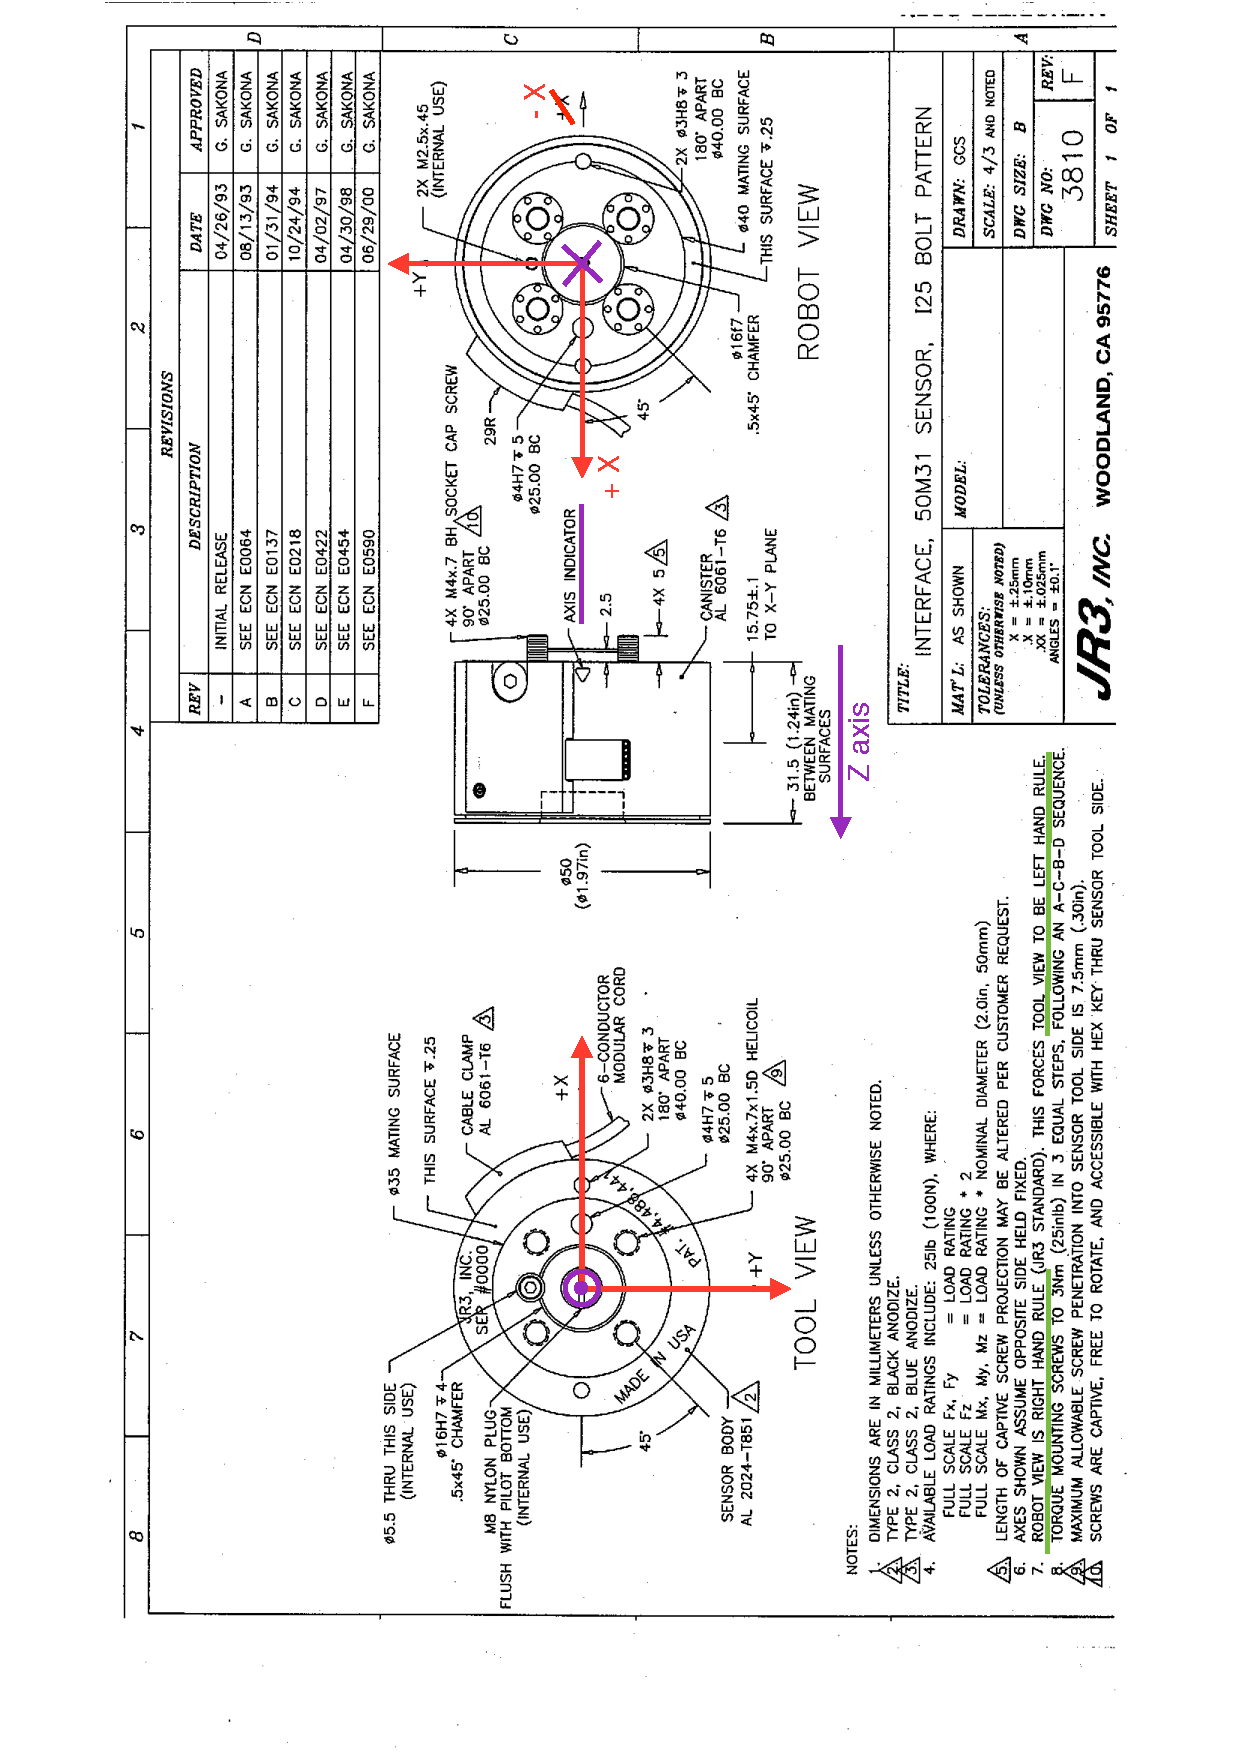
\includepdf[scale=0.8,pagecommand=\section{Información sensores JR3}\label{aped.B}]{apendices/Jr3_50M31_corregido}



\includepdf[scale=0.8,pages=2,pagecommand=\section{Información sensor IMU}\label{aped.C}]{apendices/0referencia_inercial_mti_ahrs}

\includepdf[scale=0.8,pages=3]{apendices/0referencia_inercial_mti_ahrs}

\section{Interfaz gráfiza del ZMP con sensores fuerza-par}\label{aped.D}

Se ha llevado a cabo una representación gráfica del ZMP desarrollado con el modelo de péndulo invertido simple. Ésta ha sido desarrollada en python, ya que es un lenguaje que permite la simplificación del código.

\begin{itemize}

\item \textbf{Interfaz gráfica}

\begin{figure}[H]
\centering
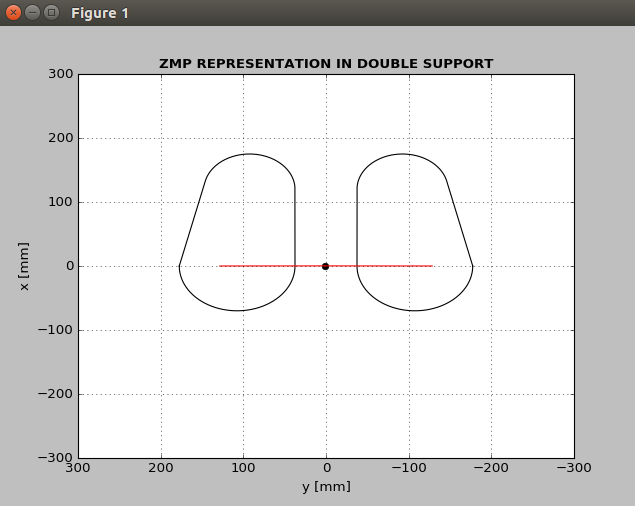
\includegraphics[scale=0.5]{apendices/interfaz_python}
\caption{Interfaz gráfica desarrollada en python}
\label{figura_interfaz_grafica}
\end{figure}

\item \textbf{Procedimiento para iniciar el programa}

Para iniciar el programa y poder visualizar los datos de manera más gráfica, se tienen que seguir los siguientes pasos:

\textbf{Paso 1}: Iniciamos una terminal (\textsc{terminal 1}), y ponemos

- ssh locomotion

- launchLocomotion 

\textbf{Paso 2}: En otra terminal (\textsc{terminal 2}) tecleamos

- ssh manipulation

- launchManipulation

Y para iniciar los sensores JR3, en esta misma consola teclear

- yarpdev --device Jr3 --period 20 --name /jr3 --ports "(ch0:o ch1:o ch2:o ch3:o)" --channels 24 --ch0:o 0 5 0 5 --ch1:o 6 11 0 5 --ch2:o 12 17 0 5 --ch3:o 18 23 0 5

\textbf{Paso 3}: Para iniciar el programa de python, abrir una nueva terminal (\textsc{terminal 3}), situarnos en la carpeta en la que esté el archivo con el código del programa y teclear

- python ZMPGraphYarpDoubleSupport.py

\end{itemize}

El código se puede obtener de: \url{https://github.com/agonzalez92/TFG}